%%%%%%%%%%%%%%%%%%%%%%%%%%%%%%%%%%%%%%%%%%%%%%%%%%%%%%%%%%%%%%%%%%%%%%%%%
%
% File: srg_operator_evolution.tex
%
% Author: A. J. Tropiano (tropiano.4@osu.edu)
% Date: May 20, 2019
%
% Notes on SRG operator evolution project.
%
% Revision history:
% 	May 31, 2019 - Renamed to srg_operator_evolution.tex from operator_evolution_May20.tex. Added a description of computing SRG unitary
%                              transformations. Added momentum projection operator contours and momentum distribution plots.                            
%
%%%%%%%%%%%%%%%%%%%%%%%%%%%%%%%%%%%%%%%%%%%%%%%%%%%%%%%%%%%%%%%%%%%%%%%%%


\documentclass[preprintnumbers,floatfix,aps,prc,preprint,nofootinbib]{revtex4-1}

% Packages
\usepackage{amsmath}
\usepackage{amsfonts}
\usepackage{amssymb}
\usepackage{bm}
\usepackage[font=small,skip=0pt]{caption} % For captions on figures and tables
\usepackage{cellspace}
\usepackage{color}
\usepackage{enumerate}
\usepackage{epsfig}
\usepackage[figuresright]{rotating}
\usepackage{float}
\usepackage{hyperref} % For clickable links to sections within table of contents
\usepackage{graphicx}
\graphicspath{{Figures/}} % Setting the graphics path
\usepackage{physics} % For bra-ket notation
\usepackage{siunitx}
\usepackage[caption=false]{subfig} % For sub-figures

\newcommand{\eps}{\varepsilon}


\begin{document}


%%%%%%%%%%%%%%%%%%%%%%%%%%%%%%%%%%%%%%%%%%%%%%%%%%%%%%%%%%%%%%%%%%%%%%%%%
\title{SRG operator evolution}


\author{A.~J.~Tropiano$^{1}$, S.~K.~Bogner$^{2}$, R.~J.~Furnstahl$^{1}$}

\affiliation{
		$^1$\mbox{Department of Physics, The Ohio State University, Columbus, OH 43210, USA}  \\
		$^2$\mbox{National Superconducting Cyclotron Laboratory and Department of Physics and Astronomy,}  \\
		\mbox{Michigan State University, East Lansing, MI 48824, USA}
}

\date{\today}

\begin{abstract}

Brief description of project.

\end{abstract}


\maketitle

\newpage


%%%%%%%%%%%%%%%%%%%%%%%%%%%%%%%%%%%%%%%%%%%%%%%%%%%%%%%%%%%%%%%%%%%%%%%%%
\section{Introduction}
\label{sec:intro}


Results on SRG-evolved operators from several NN potentials:
\\
-- How operators evolve from band- and block-diagonal SRG transformations.
\\
-- Operator evolution for different potentials (regulators, chiral order, etc.)


%%%%%%%%%%%%%%%%%%%%%%%%%%%%%%%%%%%%%%%%%%%%%%%%%%%%%%%%%%%%%%%%%%%%%%%%%
\section{Building SRG unitary transformations}
\label{sec:srg_unitary_transformations}


Brief description of how to make $U(s)$.
\\

Diagonalize initial and evolved Hamiltonians which we will call $H(0)$ and $H(s)$, respectively. This gives $\psi_{\alpha}(0)$ and $\psi_{\alpha}(s)$ for each eigenvalue indexed by $\alpha$. Then the SRG unitary transformation can be computed by taking a sum over outer products of the evolved and initial wave functions:

\begin{eqnarray}
	\label{eq:unitary_transformation}
	U(s) = \sum_{\alpha=1}^{N} \ket{\psi_{\alpha}(s)} \bra{\psi_{\alpha}(0)},
\end{eqnarray}

where N is the dimension of the Hamiltonian matrix. Here the weights are factored into the wave functions, thus $U(s)$ is unitless.
\\

To evolve operators, we simply apply $U(s)$:

\begin{eqnarray}
	\label{eq:evolved_operator}
	O(s) = U(s) O(0) U^{\dagger}(s),
\end{eqnarray}

where $O(0)$ is the bare operator.


%%%%%%%%%%%%%%%%%%%%%%%%%%%%%%%%%%%%%%%%%%%%%%%%%%%%%%%%%%%%%%%%%%%%%%%%%
\section{Operator evolution}
\label{sec:operator_evolution}


Organize this according to the figures: what story do the figures tell? Format should be description of the calculation, followed by the figure, followed by takeaways.
\\

Add the following figures: momentum projection operator figures with accompanying momentum distributions for SRG transformations from N$^3$LO non-local potential \cite{Entem:2003ft}, N$^3$LO or N$^4$LO semi-local potentials \cite{Reinert:2017usi}, and N$^2$LO local potentials \cite{Gezerlis:2014zia}.
\\

% Entem-Machleidt N3LO results

\begin{figure}[H]
	\centering
	\subfloat[]{%
	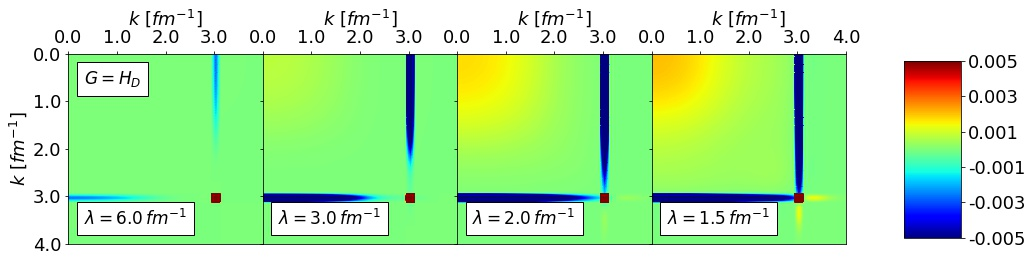
\includegraphics[clip,width=0.9\columnwidth]{momentum_projection_contours_q3,00_kvnn10_3S1_Wegner}%
	}
	
	\subfloat[]{%
	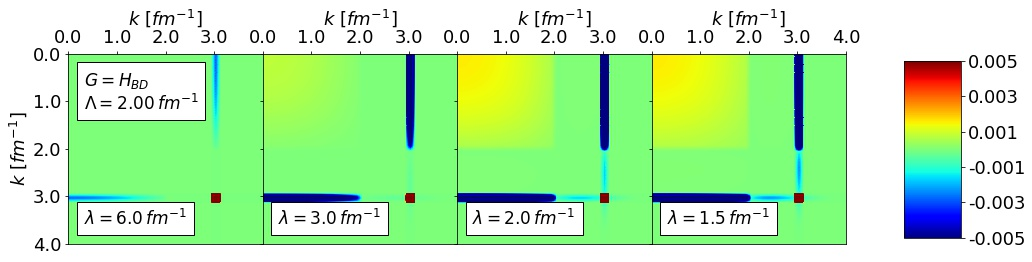
\includegraphics[clip,width=0.9\columnwidth]{momentum_projection_contours_q3,00_kvnn10_3S1_Block-diag2,00}%
	}

	\subfloat[]{%
	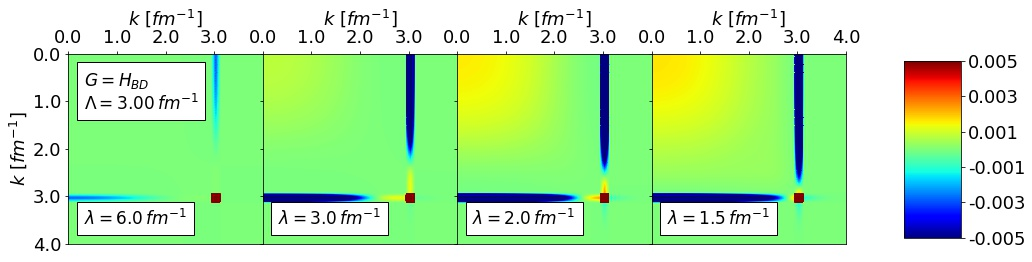
\includegraphics[clip,width=0.9\columnwidth]{momentum_projection_contours_q3,00_kvnn10_3S1_Block-diag3,00}%
	}
	\caption{Matrix elements of $\mel{k}{a^{\dagger}_q a_q}{k'}$ SRG-evolving in $\lambda$ right to left under transformations from the Entem-Machleidt N$^3$LO non-local potential with the Wegner generator (a) and block-diagonal generators decoupling at $\Lambda=2$ and $3$ fm$^{-1}$ (b and c). Here $q=3$ fm$^{-1}$.}
	\label{momentum_projection_contours_q3,00_kvnn10}
\end{figure}

\begin{figure}[H]
	\centering
	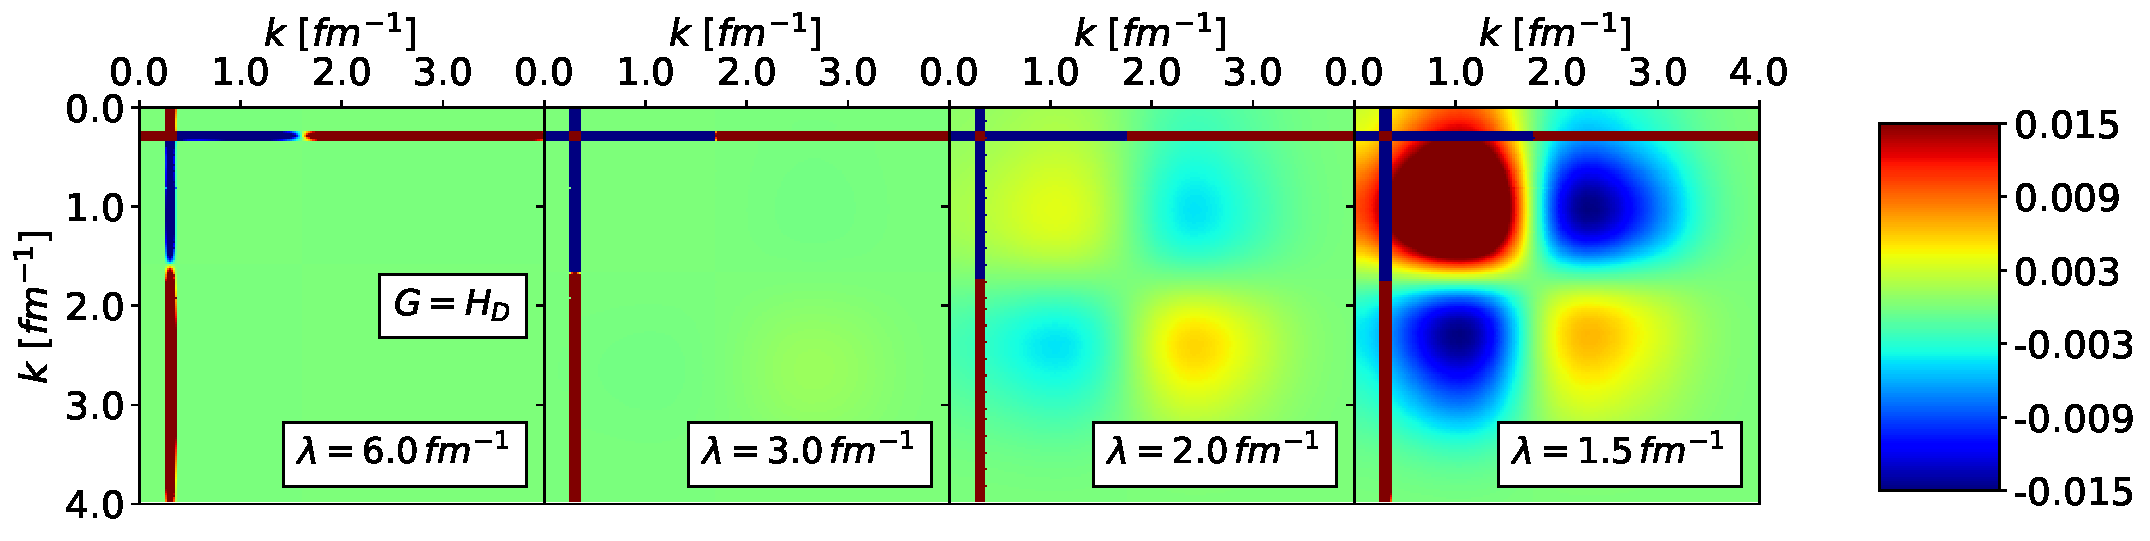
\includegraphics[clip,width=0.9\columnwidth]{momentum_projection_contours_q0,30_kvnn10_3S1_Wegner}
	\caption{Matrix elements of $\mel{k}{a^{\dagger}_q a_q}{k'}$ SRG-evolving in $\lambda$ right to left under transformations from the Entem-Machleidt N$^3$LO non-local potential with the Wegner generator. Here $q=0.3$ fm$^{-1}$.}
	\label{momentum_projection_contours_q0,30_kvnn10}
\end{figure}

\begin{figure}[H]
	\centering
	\subfloat[]{%
	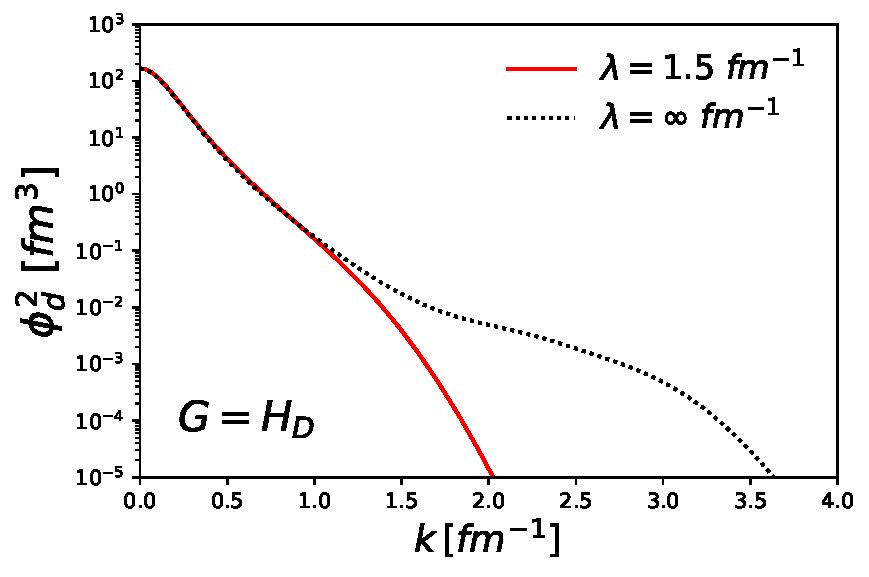
\includegraphics[clip,width=0.3\columnwidth]{deuteron_momentum_distribution_kvnn10_Wegner_lamb1,5}%
	}
	\quad
	\subfloat[]{%
	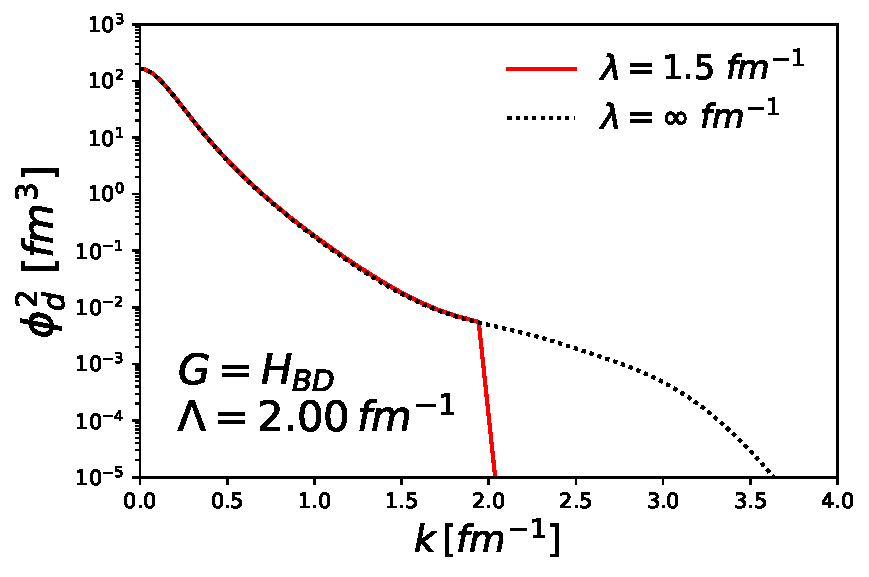
\includegraphics[clip,width=0.3\columnwidth]{deuteron_momentum_distribution_kvnn10_Block-diag2,00_lamb1,5}%
	}
	\quad
	\subfloat[]{%
	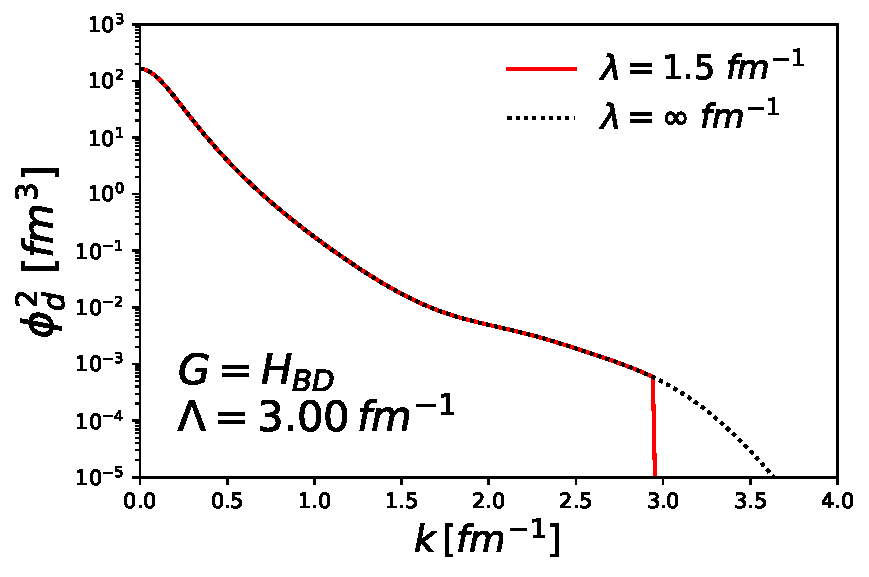
\includegraphics[clip,width=0.3\columnwidth]{deuteron_momentum_distribution_kvnn10_Block-diag3,00_lamb1,5}%
	}
	\caption{Momentum probability densities of the deuteron SRG-evolving the wave function to $\lambda=1.5$ fm$^{-1}$ from the Entem-Machleidt N$^3$LO non-local potential with the Wegner generator (a) and block-diagonal generators decoupling at $\Lambda=2$ and $3$ fm$^{-1}$ (b and c). The black dotted line corresponds to the momentum probability density of the initial deuteron wave function.}
	\label{deuteron_momentum_distribution_kvnn10}
\end{figure}

\begin{figure}[H]
	\centering
	\subfloat[]{%
	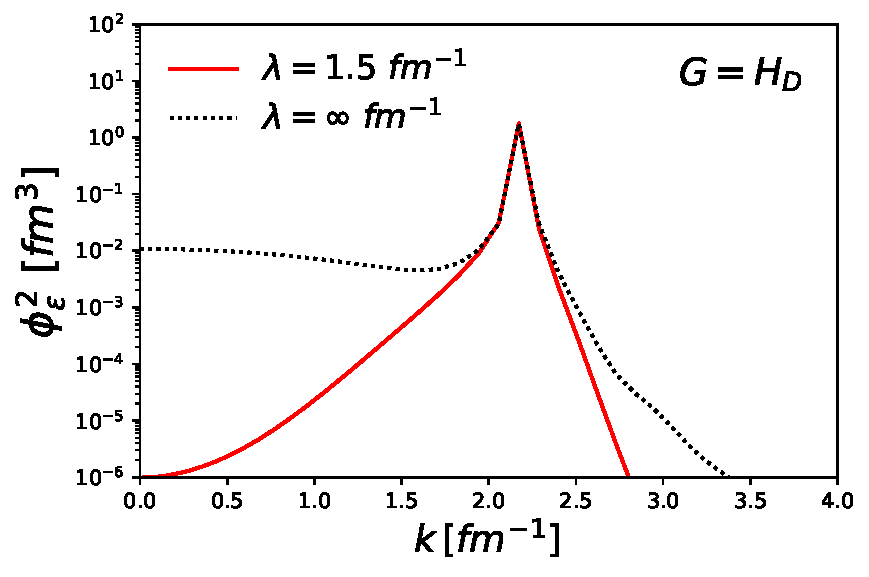
\includegraphics[clip,width=0.3\columnwidth]{continuum_state_momentum_distribution_eps200,0_kvnn10_Wegner_lamb1,5}%
	}
	\quad
	\subfloat[]{%
	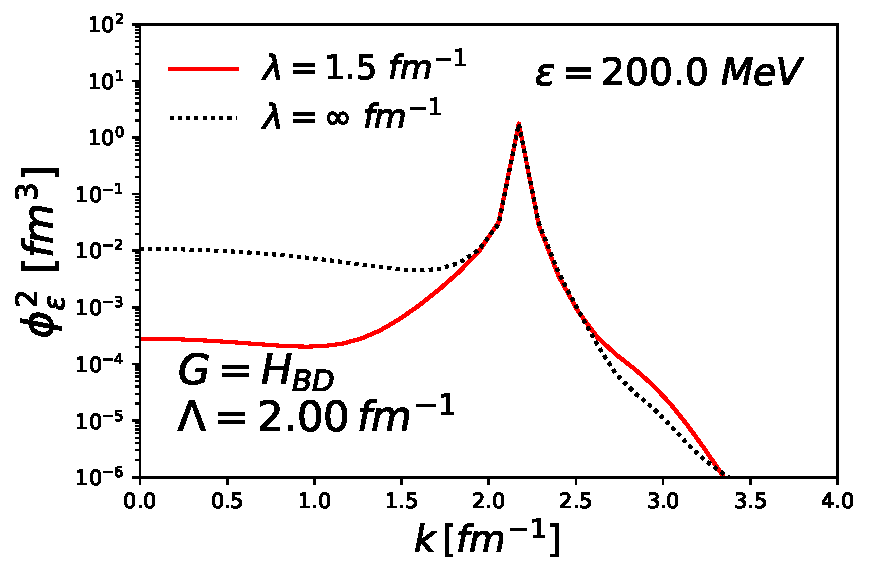
\includegraphics[clip,width=0.3\columnwidth]{continuum_state_momentum_distribution_eps200,0_kvnn10_Block-diag2,00_lamb1,5}%
	}
	\quad
	\subfloat[]{%
	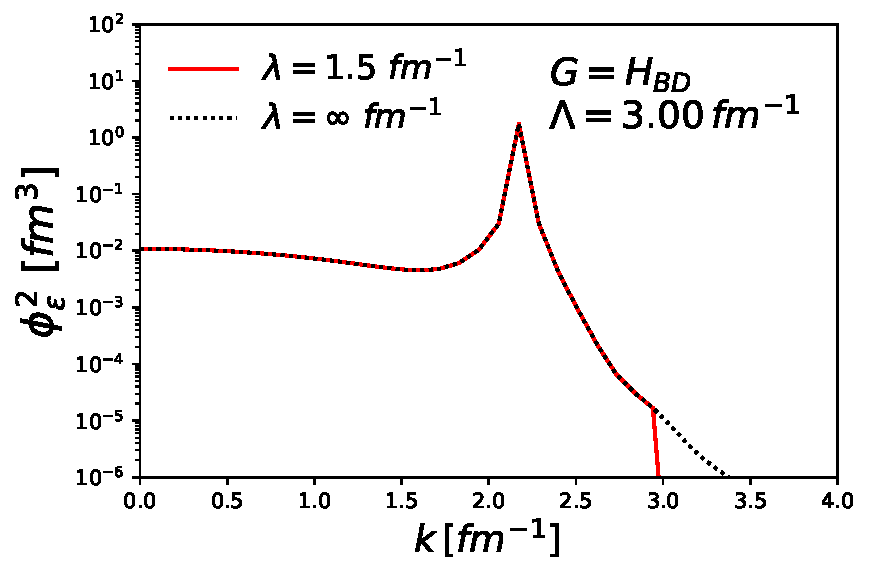
\includegraphics[clip,width=0.3\columnwidth]{continuum_state_momentum_distribution_eps200,0_kvnn10_Block-diag3,00_lamb1,5}%
	}
	\caption{Momentum probability densities of the continuum state at $\epsilon \approx 200$ MeV SRG-evolving the wave function to $\lambda=1.5$ fm$^{-1}$ from the Entem-Machleidt N$^3$LO non-local potential with the Wegner generator (a) and block-diagonal generators decoupling at $\Lambda=2$ and $3$ fm$^{-1}$ (b and c). The black dotted line corresponds to the initial momentum probability density.}
	\label{continuum_state_momentum_distribution_eps200,0_kvnn10}
\end{figure}


% RKE N3LO results

\begin{figure}[H]
	\centering
	\subfloat[]{%
	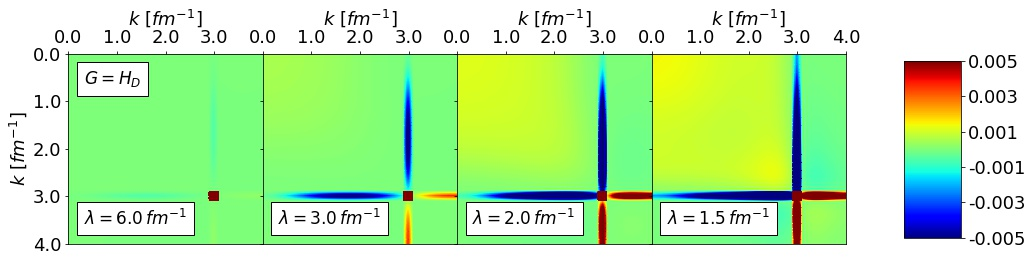
\includegraphics[clip,width=0.9\columnwidth]{momentum_projection_contours_q3,00_kvnn106_3S1_Wegner}%
	}
	
	\subfloat[]{%
	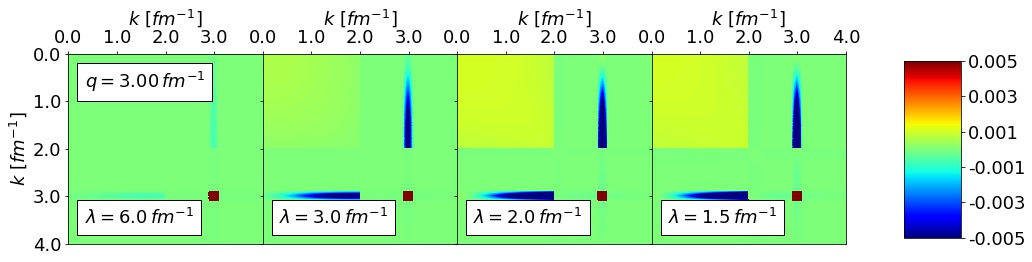
\includegraphics[clip,width=0.9\columnwidth]{momentum_projection_contours_q3,00_kvnn106_3S1_Block-diag2,00}%
	}
	\caption{Matrix elements of $\mel{k}{a^{\dagger}_q a_q}{k'}$ SRG-evolving in $\lambda$ right to left under transformations from the RKE N$^3$LO semi-local potential with the Wegner generator (a) and block-diagonal generator decoupling at $\Lambda=2$ fm$^{-1}$ (b). Here $q=3$ fm$^{-1}$ and the EFT cutoff is $450$ MeV.}
	\label{momentum_projection_contours_q3,00_kvnn106}
\end{figure}

\begin{figure}[H]
	\centering
	\subfloat[]{%
	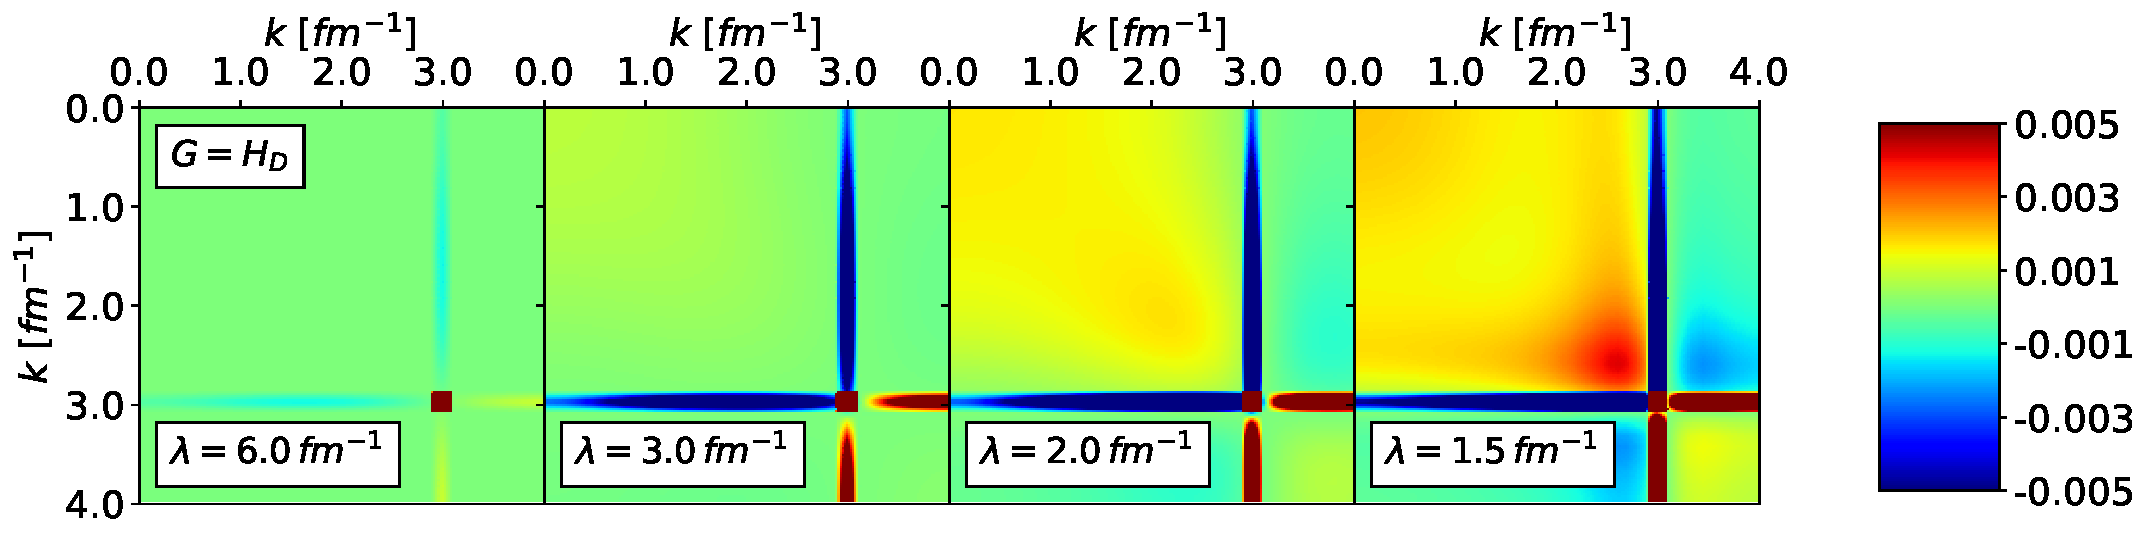
\includegraphics[clip,width=0.9\columnwidth]{momentum_projection_contours_q3,00_kvnn107_3S1_Wegner}%
	}
	
	\subfloat[]{%
	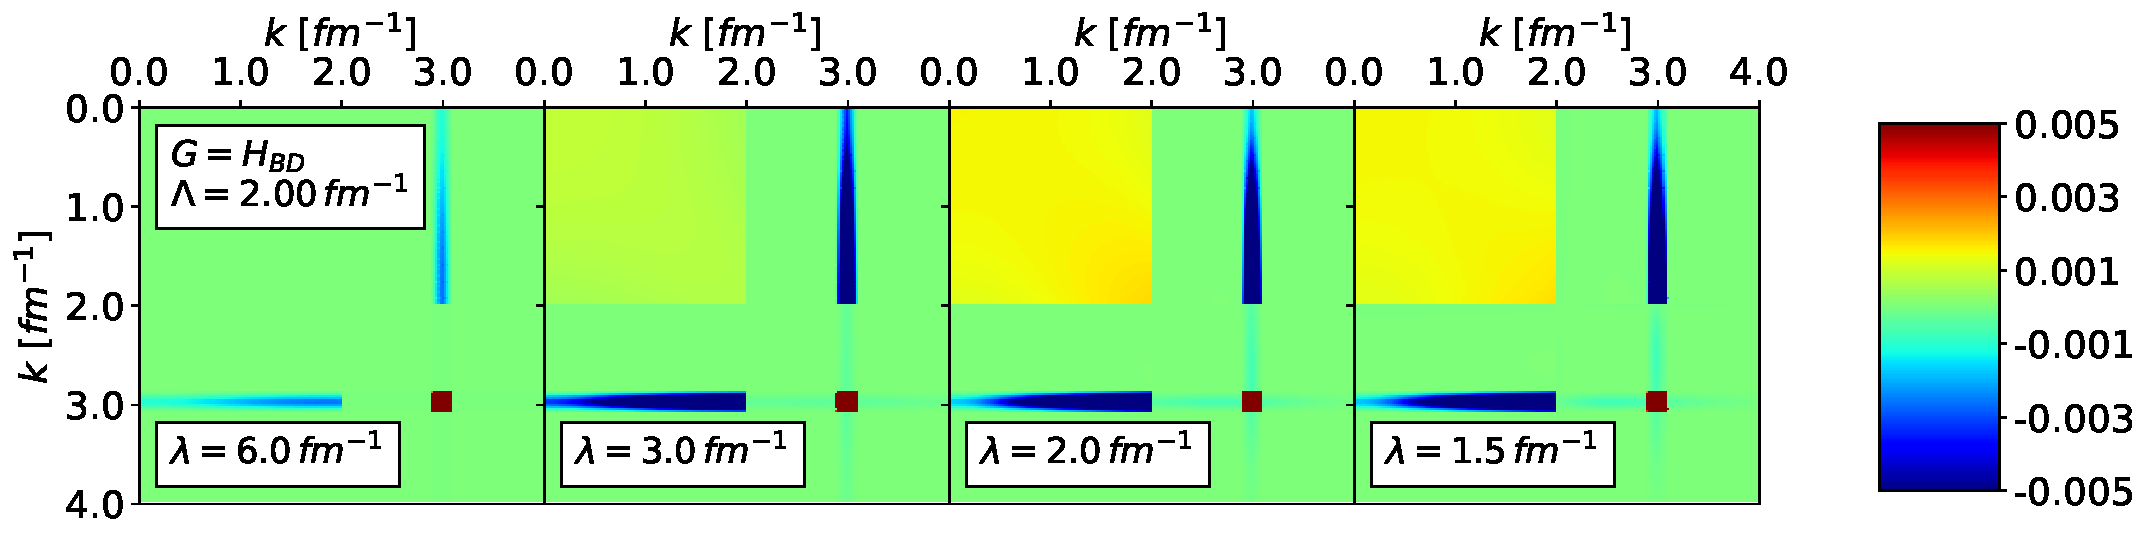
\includegraphics[clip,width=0.9\columnwidth]{momentum_projection_contours_q3,00_kvnn107_3S1_Block-diag2,00}%
	}
	\caption{Matrix elements of $\mel{k}{a^{\dagger}_q a_q}{k'}$ SRG-evolving in $\lambda$ right to left under transformations from the RKE N$^3$LO semi-local potential with the Wegner generator (a) and block-diagonal generator decoupling at $\Lambda=2$ fm$^{-1}$ (b). Here $q=3$ fm$^{-1}$ and the EFT cutoff is $500$ MeV.}
	\label{momentum_projection_contours_q3,00_kvnn107}
\end{figure}


% RKE N4LO results

\begin{figure}[H]
	\centering
	\subfloat[]{%
	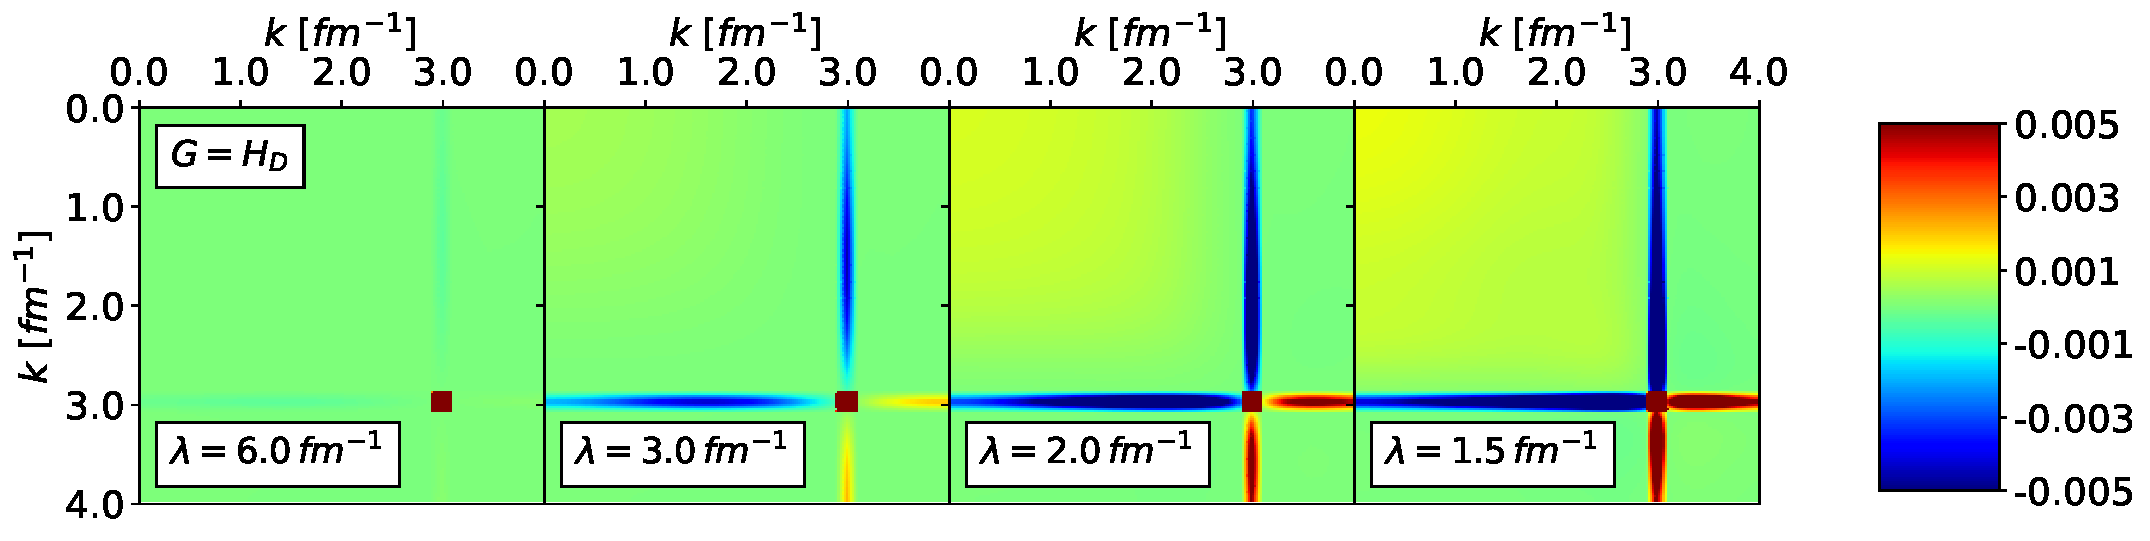
\includegraphics[clip,width=0.9\columnwidth]{momentum_projection_contours_q3,00_kvnn111_3S1_Wegner}%
	}
	
	\subfloat[]{%
	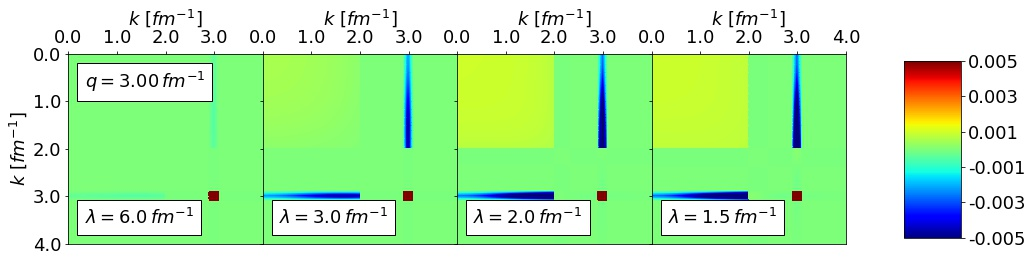
\includegraphics[clip,width=0.9\columnwidth]{momentum_projection_contours_q3,00_kvnn111_3S1_Block-diag2,00}%
	}
	\caption{Matrix elements of $\mel{k}{a^{\dagger}_q a_q}{k'}$ SRG-evolving in $\lambda$ right to left under transformations from the RKE N$^4$LO semi-local potential with the Wegner generator (a) and block-diagonal generator decoupling at $\Lambda=2$ fm$^{-1}$ (b). Here $q=3$ fm$^{-1}$ and the EFT cutoff is $450$ MeV.}
	\label{momentum_projection_contours_q3,00_kvnn111}
\end{figure}

\begin{figure}[H]
	\centering
	\subfloat[]{%
	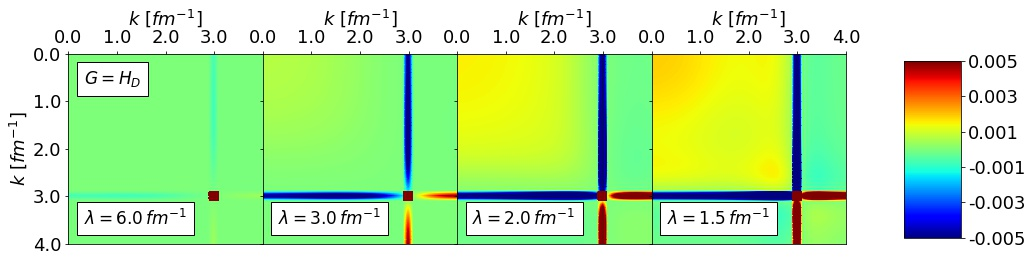
\includegraphics[clip,width=0.9\columnwidth]{momentum_projection_contours_q3,00_kvnn112_3S1_Wegner}%
	}
	
	\subfloat[]{%
	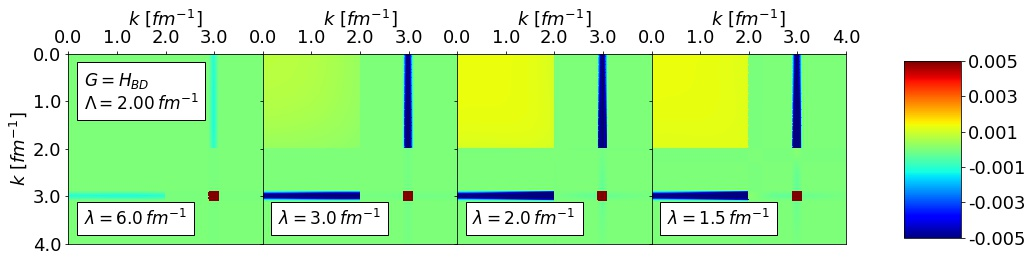
\includegraphics[clip,width=0.9\columnwidth]{momentum_projection_contours_q3,00_kvnn112_3S1_Block-diag2,00}%
	}
	\caption{Matrix elements of $\mel{k}{a^{\dagger}_q a_q}{k'}$ SRG-evolving in $\lambda$ right to left under transformations from the RKE N$^4$LO semi-local potential with the Wegner generator (a) and block-diagonal generator decoupling at $\Lambda=2$ fm$^{-1}$ (b). Here $q=3$ fm$^{-1}$ and the EFT cutoff is $500$ MeV.}
	\label{momentum_projection_contours_q3,00_kvnn112}
\end{figure}

\begin{figure}[H]
	\centering
	\subfloat[]{%
	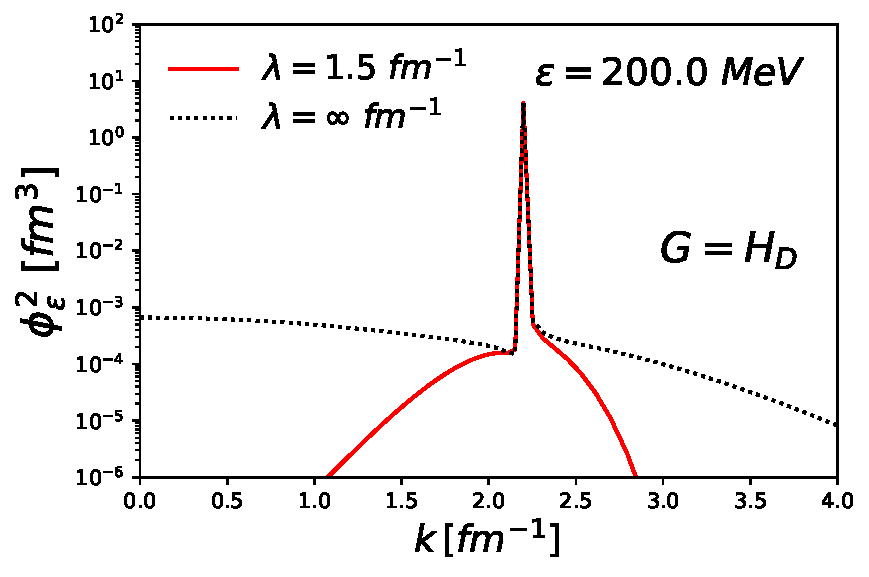
\includegraphics[clip,width=0.3\columnwidth]{continuum_state_momentum_distribution_eps200,0_kvnn111_Wegner_lamb1,5}%
	}
	\quad
	\subfloat[]{%
	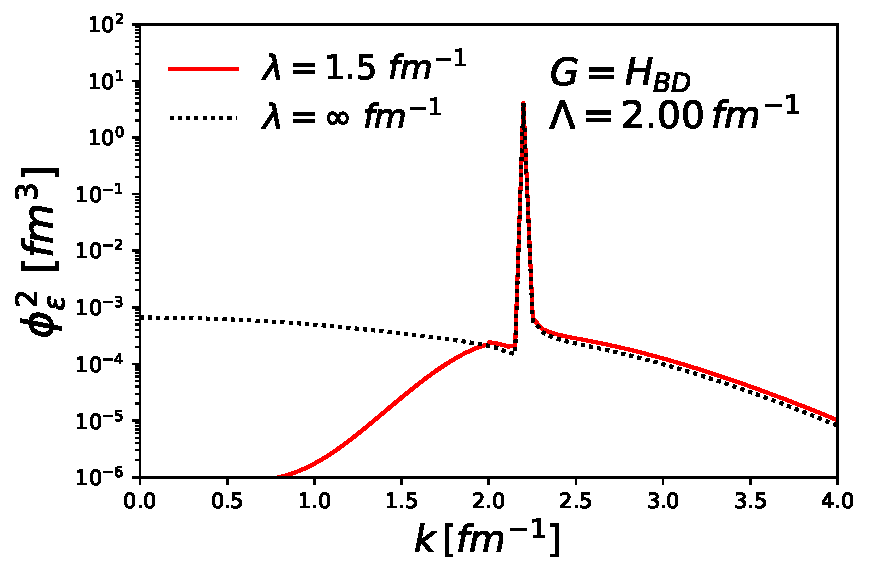
\includegraphics[clip,width=0.3\columnwidth]{continuum_state_momentum_distribution_eps200,0_kvnn111_Block-diag2,00_lamb1,5}%
	}
	\quad
	\subfloat[]{%
	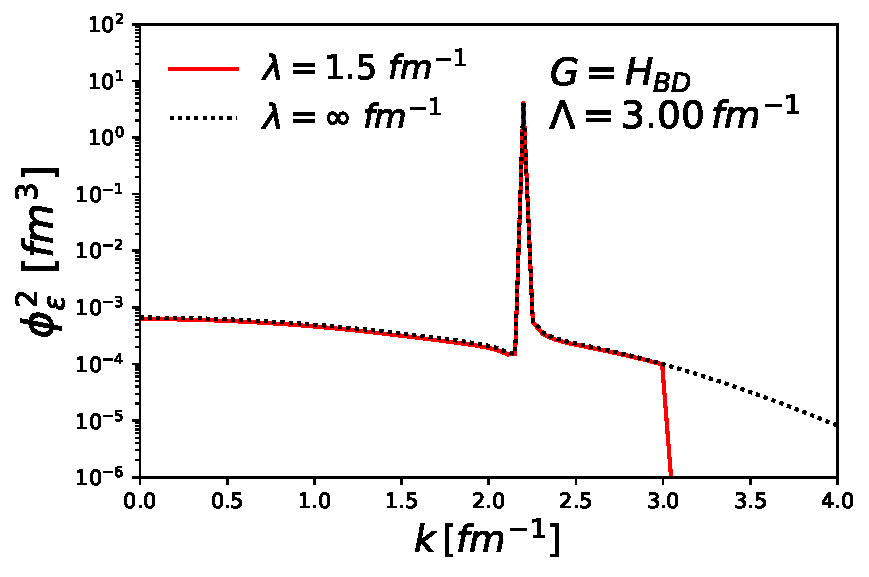
\includegraphics[clip,width=0.3\columnwidth]{continuum_state_momentum_distribution_eps200,0_kvnn111_Block-diag3,00_lamb1,5}%
	}
	\caption{Momentum probability densities of the continuum state at $\epsilon \approx 200$ MeV SRG-evolving the wave function to $\lambda=1.5$ fm$^{-1}$ from the RKE N$^4$LO semi-local potential with the Wegner generator (a) and block-diagonal generators decoupling at $\Lambda=2$ and $3$ fm$^{-1}$ (b and c). The black dotted line corresponds to the initial momentum probability density. Here the EFT cutoff is $450$ MeV.}
	\label{continuum_state_momentum_distribution_eps200,0_kvnn111}
\end{figure}

% Gez. et al. N2LO results

\begin{figure}[H]
	\centering
	\subfloat[]{%
	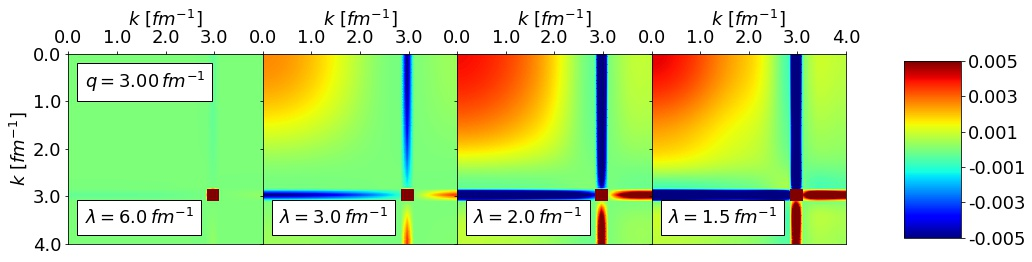
\includegraphics[clip,width=0.9\columnwidth]{momentum_projection_contours_q3,00_kvnn222_3S1_Wegner}%
	}
	
	\subfloat[]{%
	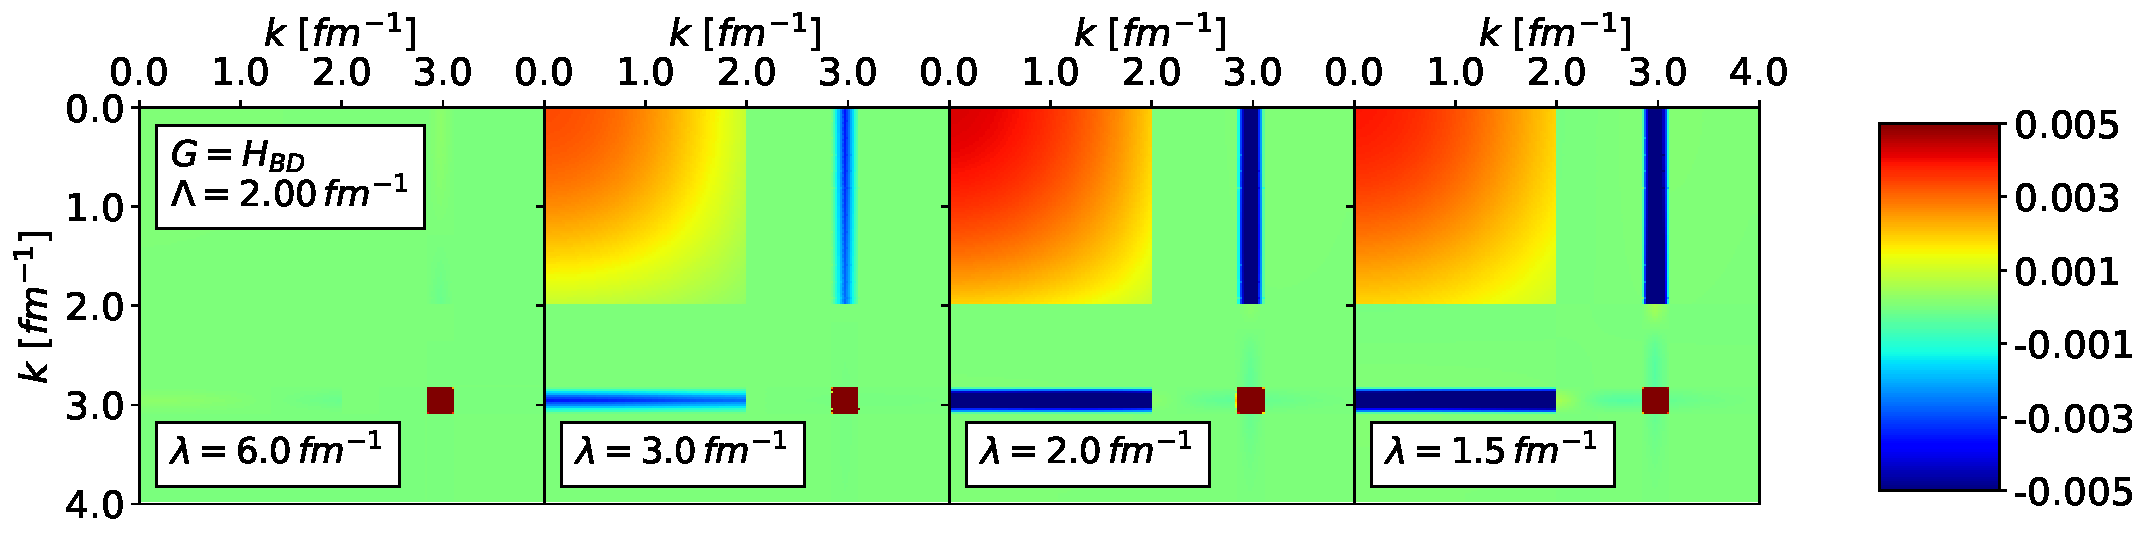
\includegraphics[clip,width=0.9\columnwidth]{momentum_projection_contours_q3,00_kvnn222_3S1_Block-diag2,00}%
	}

	\subfloat[]{%
	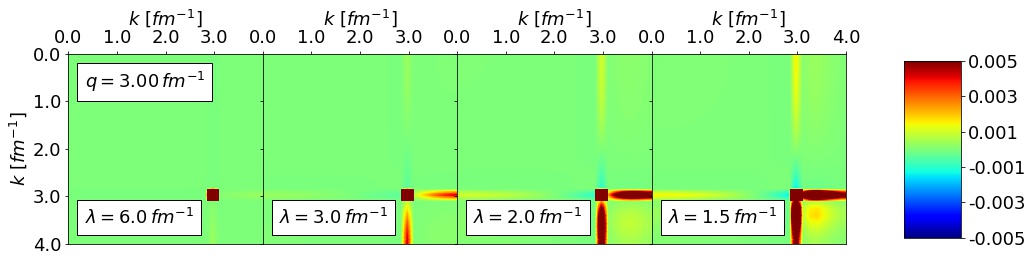
\includegraphics[clip,width=0.9\columnwidth]{momentum_projection_contours_q3,00_kvnn222_3S1_Block-diag3,00}%
	}
	\caption{Matrix elements of $\mel{k}{a^{\dagger}_q a_q}{k'}$ SRG-evolving in $\lambda$ right to left under transformations from the Gezerlis et al. N$^2$LO local potential with the Wegner generator (a) and block-diagonal generators decoupling at $\Lambda=2$ and $3$ fm$^{-1}$ (b and c). Here $q=3$ fm$^{-1}$ and the EFT cutoff is $1$ fm.}
	\label{momentum_projection_contours_q3,00_kvnn222}
\end{figure}

\begin{figure}[H]
	\centering
	\subfloat[]{%
	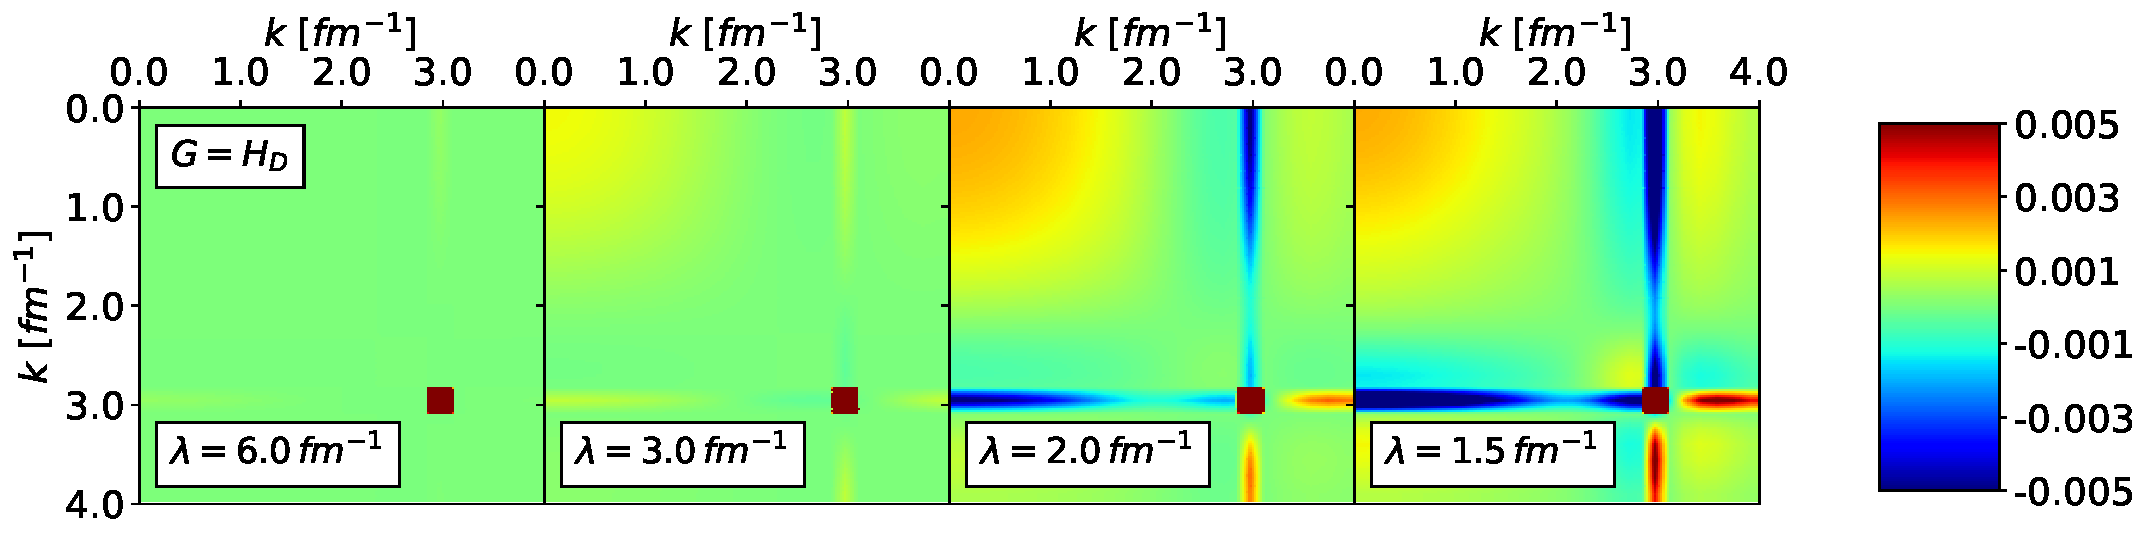
\includegraphics[clip,width=0.9\columnwidth]{momentum_projection_contours_q3,00_kvnn224_3S1_Wegner}%
	}
	
	\subfloat[]{%
	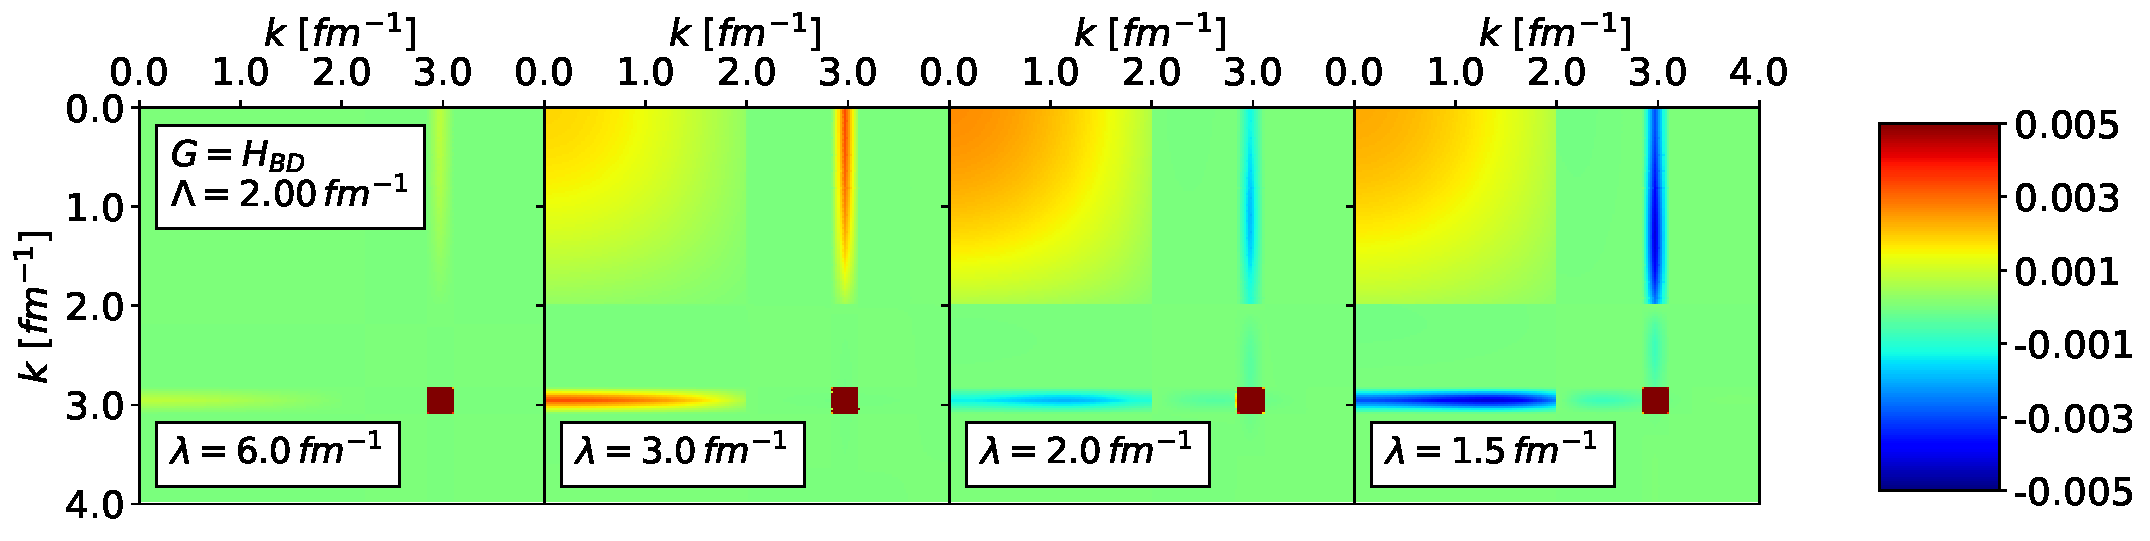
\includegraphics[clip,width=0.9\columnwidth]{momentum_projection_contours_q3,00_kvnn224_3S1_Block-diag2,00}%
	}
	\caption{Matrix elements of $\mel{k}{a^{\dagger}_q a_q}{k'}$ SRG-evolving in $\lambda$ right to left under transformations from the Gezerlis et al. N$^2$LO local potential with the Wegner generator (a) and block-diagonal generator decoupling at $\Lambda=2$ fm$^{-1}$ (b). Here $q=3$ fm$^{-1}$ and the EFT cutoff is $1.2$ fm.}
	\label{momentum_projection_contours_q3,00_kvnn224}
\end{figure}


%%%%%%%%%%%%%%%%%%%%%%%%%%%%%%%%%%%%%%%%%%%%%%%%%%%%%%%%%%%%%%%%%%%%%%%%%


\bibliography{../tropiano_bib}


\end{document}